\documentclass[twocolumn,article,amsmath,amssymb,floatfix,aps]{revtex4}
\usepackage{graphicx}
\usepackage{epsfig}
\usepackage{multirow}
\usepackage{color}
\usepackage{cancel}



\begin{document}

\title{Parity Partner Bands in $^{163}$Lu: \\ A novel approach for describing the negative parity states from a triaxial super-deformed band}% Force line breaks with \\

\author{R.  Poenaru}%
 \email{robert. poenaru@drd. unibuc. ro}
 \affiliation{Doctoral School of Physics, University of Bucharest}%
 \affiliation{Horia Hulubei National Institute of Nuclear Physics and Engineering, Magurele}%
\author{A.  A.  Raduta}%
\email{raduta@nipne. ro}
\affiliation{Horia Hulubei National Institute of Nuclear Physics and Engineering, Magurele}%
\affiliation{Academy of Romanian Scientists, Bucharest}%

\date{\today}

\begin{abstract}
 The wobbling spectrum of $^{163}$Lu is described through a novel approach, starting from a triaxial rotor model within a semi-classical picture, and obtaining a new set of equations for all four rotational bands that have wobbling character.  Redefining the band structure in the present model is done by adopting the concepts of Signature Partner Bands and Parity Partner Bands.  Indeed, describing a wobbling spectrum in an even-odd nucleus through signature and parity quantum numbers is an inedited interpretation of the triaxial super-deformed  bands. 

\end{abstract}

\maketitle


%\section{Introduction}
 The wobbling motion was first described by Bohr and Mottelson within a particle triaxial rotor coupling, where the rotation axis moves on a curly cone.  This sort of motion is a signature of the triaxial nuclei, these being not much considered across the time. 
Although it was firstly predicted theoretically for even-even nuclei \cite{BMott}, this collective mode was also pointed out in several even-odd nuclei, with $^{163}$Lu being considered the best \emph{wobbler}, mainly due to its relatively rich spectrum: four triaxial super-deformed bands $TSD_{1,2,3,4}$.   The $TSD_1$ is interpreted as the ground state - yrast - band, while the other three as  wobbling multi-phonon excited bands \cite{odegaard2001evidence,Jens}. The common view on these bands is that the alignment of the odd-proton angular momentum, $i_{13/2}$ drives the system  to very large stable deformation.  In the meantime, several neighboring odd-nuclei were identified as wobblers i. e. , $^{161,165,167}$Lu \cite{Jens,Scho,Amro,Hage,Bring,Hage1},,and recently the nuclei $^{135}$Pr \cite{Matta,Sen}, $^{167}$Ta \cite{Bring,Hart}, $^{187}$Au \cite{Sen1}, $^{130}$Ba\cite{Chen}, $^{105}$Pd \cite{Timar}, 
$^{127}$Xe \cite{Chakr}, and $^{183}$Au \cite{Nand}. 


In  a previous work \cite{raduta2020towards,raduta2020new}, a successful  description of the wobbling phenomenon in $^{163}$Lu was achieved.  Therein, the calculations were based on a particle-triaxial rotor system, that was semi-classically treated. 
The band structure was obtained in terms of two ground state bands (TSD1 and TSD2) of different signatures, given by  coupling  an odd $j=i_{13/2}$ proton to a core with angular momenta R=0,2,4,6,. .  and R=1,3,5,. . . , respectively, one wobbling phonon excitation  of the TSD2 band, $n_w=1$, $TSD_3$, and one ground state band obtained by coupling  a different valence nucleon, namely the $j=h_{9/2}$ to a core exhibiting an a. m.  from the sequence $\mathbf{R}=0,2,4,\dots$.  

Here we address the question whether the four TSD bands could be described by coupling a unique single particle state, i. e.  $i_{13/2}$, to a core of a natural parity for $TSD_{1,2,3}$ and a core of negative parity and $\mathbf{R}=1,3,5,\dots$.  in the case of $TSD_4$.  Within this particle-core basis a similar Hamiltonian as in the previous paper is treated via a time dependent variational formalism.  In this manner one derives the classical equations of motion for the generalized canonical coordinates. 

For the sake of a self content presentation,in what follows we shall briefly introduce the necessary ingredients of the formalism.  

The Hamiltonian of $^{163}$Lu has a particle-rotor character and describes the interaction between an even-even triaxial core and a single nucleon that moves in the quadrupole deformed mean field generated by the core. 

\begin{align}
    H=H_\text{rot}+H_\text{sp}\ .  \label{hamiltonian_formula}
\end{align}

The first term represents the triaxial rotor Hamiltonian, with the core a. m.  $\mathbf{R}=\mathbf{I}-\mathbf{j}$, and the inertial parameters $A_k$. 

\begin{align}
    H_\text{rot}=\sum_{i=1,2,3}A_i\left(I_i-j_i\right)^2,
\end{align}
 
 The inertial parameters $A_i$ are related to the moments of inertia (MoI)corresponding to the principal axes of the triaxial ellipsoid, through the equation $A_i=\frac{1}{2\mathcal{I}_i}$.  

The single-particle term from Eq.  \ref{hamiltonian_formula} is defined in terms of the triaxiality parameter $\gamma$ and the potential strength $V$. Actually  this term expresses the mean field for the single particle motion, determined by a collective quadrupole and a single particle quadrupole interaction \cite{Davyd}. 

\begin{align}
    H_\text{sp} = \frac{V}{j(j+1}\left[\cos\gamma\left(3j_3^2-\mathbf{j}^2\right)-\sqrt{3}\sin\gamma\left(j_1^2-j_2^2\right)\right]+\epsilon_j.  \label{sp_hami}
\end{align}

The term $\epsilon_j$ from Eq.  \ref{sp_hami} represents the single particle energy. 
The eigenvalues of interest for $H$ are obtained on the base of a semi-classical approach. 
Thus, the total Hamiltonian $H$ is dequantized through  the time dependent variational equation (TDVE):
\begin{equation}
\delta\int_{0}^{t}\langle \Psi_{IjM}|H-i\frac{\partial}{\partial t'}|\Psi_{IjM}\rangle d t'=0,
\end{equation}
where the trial function is chosen as:
\begin{equation}
|\Psi_{Ij;M}\rangle ={\bf N}e^{z I_-}e^{s j_-}|IMI\rangle |jj\rangle ,
\end{equation} 
with $I_-$ and ${j}_-$ denoting the lowering operators for the intrinsic angular momenta ${\bf I}$ and ${\bf j}$ respectively, while ${\bf N}$ is  the normalization factor. 
$|IMI\rangle $ and $|jj\rangle$ are extremal states for the operators ${\hat I}^2, {\hat I}_3$ and ${\hat j}^2, {\hat j}_3$, respectively.  We notice that the trial function is a mixture of  components of definite K, which is consistent with the fact that for triaxial nuclei, $K$ is not a good quantum number.  The name of TSD bands is the abbreviation for triaxial super-deformed bands suggesting that the ground band head state is an isomeric state with a relative large half-life. 
 
The variables $z$ and $s$ are complex functions of time and play the role of classical phase space coordinates describing the motion of the core and the odd particle, respectively:
\begin{equation}
z=\rho e^{i\varphi},\;\;s=fe^{i\psi}. 
\end{equation}
Changing the variables $\rho$ and $f$ to  $ r$ and $t$, respectively:
\begin{equation}
r=\frac{2I}{1+\rho^2},\;\;0\le r\le 2I;\;\;
t=\frac{2j}{1+f^2},\;\; 0\le t\le 2j,
\end{equation}
the classical equations of motion acquire the canonical Hamilton form:
\begin{equation}
\frac{\partial {\cal H}}{\partial r}=\stackrel{\bullet}{\varphi},\;\frac{\partial {\cal H}}{\partial \varphi}=-\stackrel{\bullet}{r};\;
\frac{\partial {\cal H}}{\partial t}=\stackrel{\bullet}{\psi};\;\frac{\partial {\cal H}}{\partial \psi}=-\stackrel{\bullet}{t}.  
\label{eqmot}
\end{equation}
where ${\cal H}$ denotes the average of $H$ with the trial function $|\Psi_{IjM}\rangle$ and plays the role of the classical energy function. 
The classical energy has the expression : 
\begin{equation}
{\cal H}(r,\varphi;t,\psi)=\langle \Psi_{IjM}|H|\Psi_{IjM}\rangle\nonumber\\
\label{classen}
\end{equation} 
and is minimal (${\cal H}^{(I,j)}_{min}$) in the point
$(\varphi,r)=(0,I);(\psi,t)=(0,j)$, when $A_1<A_2<A_3$.   
Linearizing the equations of motion around the minimum point of ${\cal H}$, one obtains a harmonic motion for the system, with the frequency given by the equation:
\begin{equation}
\Omega^4+B\Omega^2+C=0,
\label{ecOm}
\end{equation}
where the coefficients B and C have the expressions:
\begin{widetext}
%\begin{scriptsize}
\begin{eqnarray}
&&-B=\left[(2I-1)(A_3-A_1)+2jA_1\right]\left[(2I-1)(A_2-A_1)+2jA_1\right]+8A_2A_3Ij\\
 &+&\left[(2j-1)(A_3-A_1)+2IA_1+V\frac{2j-1}{j(j+1)}\sqrt{3}(\sqrt{3}\cos\gamma+\sin\gamma)\right]
 \left[(2j-1)(A_2-A_1)+2IA_1+V\frac{2j-1}{j(j+1)}2\sqrt{3}\sin\gamma\right],\nonumber\\
&&C=\left\{\left[(2I-1)(A_3-A_1)+2jA_1\right]\left[(2j-1)(A_3-A_1)+2IA_1+V\frac{2j-1}{j(j+1)}\sqrt{3}(\sqrt{3}\cos\gamma+\sin\gamma)\right]
- 4IjA_3^2\right \}\nonumber\\
 &\times&\left\{\left[(2I-1)(A_2-A_1)+2jA_1\right]\left[(2j-1)(A_2-A_1)+2IA_1+V\frac{2j-1}{j(j+1)}2\sqrt{3}\sin\gamma\right]-4IjA_2^2\right\}. 
\label{BandC}
\end{eqnarray}
%\end{scriptsize}
\end{widetext}
Under certain restrictions for MoI's the dispersion equation (\ref{ecOm}) admits two real and positive solutions, which here after  will be denoted by $\Omega^{I}_1$ and $\Omega^{I}_{2}$ for $j=i_{13/2}$and ordered as: $\Omega^I_1<\Omega^I_{2}$ . 

Further, to the $TSD_{1,2,3,4}$ bands we associate the energies:
%\begin{scriptsize}
\begin{eqnarray}
  &&  E_I^\text{TSD1}=\epsilon_{j} + \mathcal{H}_\text{min}^{(I,j)}+\mathcal{F}_{00}^I , \;\;I=R+j, R=0,2,4,. . . ,\nonumber \\
  &&  E_I^\text{TSD2}=\epsilon_{j,1} + \mathcal{H}_\text{min}^{(I,j)}+\mathcal{F}_{00}^I , \;\;I=R+j, R=1,3,5,. . . \nonumber\\
  &&  E_I^\text{TSD3}=\epsilon_{j} + \mathcal{H}_\text{min}^{(I,j)}+\mathcal{F}_{10}^I, \;\; I=R+j, R=0,2,4,. . .  \nonumber\\
  &&  E_I^\text{TSD4}=\epsilon_{j,2} + \mathcal{H}_\text{min}^{(I,j)}+\mathcal{F}_{00}^I,\;\;I=R+j,\;R=1,3,5,. . . . \nonumber\\ \label{wobbling_energies}
\end{eqnarray}
%\end{scriptsize}
where $\mathcal{F}_{n_{w_1}n_{w_2}}$ is function of the wobbling frequencies

\begin{align}
    F_{n_{w_1}n_{w_1}}^I=(n_{w_1}+\frac{1}{2})\Omega_1^I+(n_{w_2}+\frac{1}{2})\Omega_2^I.  \label{phonons}
\end{align}
while $\mathcal{H}^{(I,j)}_{min}$  is the minimal classical energy.  We considered different re-normalizations for the single-particle mean field in the signature unfavored as well as in the negative parity states, which result two distinct energy shifts for the excitation energies in the TSD2 and TSD4 bands, respectively. These two quantities will be adjusted throughout the numerical calculations such that the energy spectrum is best reproduced.  The phonon numbers corresponding to the four bands are listed in Table \ref{tabular_phonon_numbers}, where values of the parity and signatures are also shown. 
In a previous publication \cite{raduta2020new} one showed that the signature is a good quantum number. 
One can  prove that parity is also a good quantum number in our formalism.  Indeed, taking into account that the parity operator is a product of the complex conjugation operation and a rotation of angle $\pi$ around the 2-axis ($P=e^{-i\pi J_2}C$) and acting on the trial function with the total parity operator $P_t=P_cP_{sp}$ one obtains:
\begin{equation}
P_t\Psi(r,\varphi;t,\psi)=\Psi(r,\varphi+\pi; t, \psi +\pi). 
\end{equation}
On the other hand the energy function is invariant at changing the angles with $\pi$:
\begin{equation}
{\cal{H}}(r,\varphi+\pi; t, \psi +\pi)={\cal{H}}(r,\varphi;t,\psi). 
\end{equation}
This induces the fact that the functions $\Psi$ and its image through $P_t$ are linear dependent differing by a multiplicative constant of modulus equal to unity.  Thus,
\begin{equation}
\Psi(r,\varphi+\pi; t, \psi +\pi)=\pm \Psi(r,\varphi;t,\psi). 
\end{equation}
The above result is a reflection of the fact that the triaxial rotor admits eigenfunctions of negative parity.  Indeed, let $r_k$ ,k=0,1,2,3 be the eigenvlues of the four elements of the group $D_2$:
${\cal{E}},e^{-i\pi R_1}, e^{-i\pi R_2}, e^{-i\pi R_3}$ with ${\cal{E}}$ denoting the unity rotation.  The eigenfunctions of the rotor Hamiltonian being at a time  eigenfunctions for the $D_2$ elements form irreducible representation of the group, with the eigenvalues $(r_0,r_1,r_2,r_3)$.  Two of these irrep-s have negative parity.  These are: $(1, -1, -1, 1)$ and $(1, 1, -1, -1)$. 

 The spin sequences for the TSD bands are shown in Table \ref{spin_sequences}. 

\begin{table}[h]
    \centering
  \begin{tabular}{lllll}
  \hline
Band & $n_{w_1}$ & $n_{w_2}$ &  $\pi$ &  $\alpha$ \\
\hline
\hline
TSD1 &     0      &       0    &    +1  &    +1/2  \\
TSD2 &    0       &       0    &    +1  &    -1/2  \\
TSD3 &     1      &     0      &    +1  &    +1/2  \\
TSD4 &     0      &     0      &     -1  &    -1/2  \\
\hline
\end{tabular}
    \caption{The wobbling phonon numbers, parities and signatures assigned for the triaxial bands in $^{163}$Lu  within the model. }
    \label{tabular_phonon_numbers}
\end{table}

\begin{table}[h]
    \centering
  \begin{tabular}{llll}
  \hline
Band & j & $\mathbf{R}$-sequence & $\mathbf{I}$-sequence \\
\hline
\hline
TSD1 & $i_{13/2}$  &   $0,2,4,\dots$         &   $13/2,17/2,21/2,\dots$         \\
TSD2 & $i_{13/2}$  &   $1,3,5,\dots$         &           $27/2,31/2,35/2,\dots$ \\
TSD3 & $i_{13/2}$  &  $0,2,4,\dots$ & $33/2,37/2,41/2,\dots$     \\
TSD4 & $i_{13/2}$  &         $1,3,5,\dots$   &       $47/2,51/2,55/2,\dots$    
\end{tabular}
    \caption{The spin sequences that belong to the wobbling spectrum of $^{163}$Lu, where $j$ is the $i_{13/2}$-odd proton.  }
    \label{spin_sequences}
\end{table}

In what follows it is worth  analyzing  the dependence of the classical energy function on the Cartesian coordinates $x_k=I_k,\;k=1,2,3$:

\begin{equation}
    x_1=I\sin\theta \cos\varphi\ ,
    x_2=I\sin\theta \sin\varphi\ ,
    x_3=I\cos\theta. 
\end{equation}

In polar coordinates the classical energy function reads:

\begin{eqnarray}
    \mathcal{H}&=&I\left(I-\frac{1}{2}\right)\sin^2\theta\left(A_1\cos^2\varphi+A_2\sin^2\varphi-A_3\right)-\nonumber\\
    &-&2A_1Ij\sin\theta+T_{rot}+T_{sp}\ , \label{energy_function}
\end{eqnarray}
\noindent
where the last two terms are independent of the coordinates and have the forms:

\begin{align}
    T_{rot}&=\frac{I}{2}(A_1+A_2)+A_3I^2\ ,\\
    T_{sp}&=\frac{j}{2}(A_2+A_3)+A_1j^2-V\frac{2j-1}{j+1}\sin\left(\gamma+\frac{\pi}{6}\right)\ . 
\end{align}
In obtaining this expression the single particle terms were considered in the minimum point. 

The classical energy admits two constants of motion: the system energy and the total angular momentum.  Therefore, the classical trajectories are determined by intersecting the surfaces describing the two constants of motion, that are an ellipsoid and a sphere, respectively:

\begin{align}   
    E=&\left(1-\frac{1}{2I}\right)A_1x_1^2+\left(1-\frac{1}{2I}\right)A_2x_2^2\nonumber \\
      &+\left[\left(1-\frac{1}{2I}\right)A_3+A_1\frac{j}{I}\right]x_3^2 \nonumber \\
      &+T_{rot}+T_{sp}-I\left(I-\frac{1}{2}\right)A_3-2A_1Ij, \label{ellipsoid_rotation}\nonumber \\
  I^2=&x_1^2+x_2^2+x_3^3. 
\end{align}

 For a given total angular momentum and a given set of MoI's one can solve the above equations by expressing two unknowns in term of the third one and thus, classical trajectories of an wobbling character are obtained. 
%\section{Numerical results}

We  now  proceed at discussing the numerical results.  As already mentioned  the application is made for $^{163}$Lu, since this is the only isotope exhibiting both positive and negative parity bands
and thus one can check the validity of our proposed formalism. 
 By using the expressions \ref{wobbling_energies}, a least squares fitting procedure was used for finding the parameter set $\mathcal{P}=(\mathcal{I}_1,\mathcal{I}_2,\mathcal{I}_3,\gamma,V)$.  The found values of $\mathcal{P}$, are  shown in Table \ref{parameter_set},leading to a RMS value of $\approx 79$ keV, which is much better than that obtained through a different approach
 \cite{raduta2020new}, where the r. m. s.  is $\approx 240 keV$.  Keep in mind that the fitting procedure was done simultaneously for all four bands,contrary to Ref. \cite{raduta2020new}) where a separate parameter set for TSD4 was used, invoking a different polarization effect of the core, due to the particle-core interaction.  Concerning the single particle energies, the unfavored states as well as the negative parity states induce a correction for the mean field with the quantities: $\epsilon_{J,1}-\epsilon_{j}=0. 3MeV$ and $\epsilon_{J,2}-\epsilon_{j}=0. 6$ MeV respectively.  Results of our calculations are compared with the corresponding data in Fig.  \ref{tsd_bands}, where one remarks a very good agreement of the two sets of energies.  Remarkable the fact that the difference $E_I^\text{TSD4}-E_I^\text{TSD2}\approx 300 keV$, which suggests that the states of the same a. m.  from the TSD2 and TSD4 bands might emerge through the parity projection from a sole function without space reflection symmetry.  In our case, this is caused by the fact that the wobbling frequency is parity independent.  In this context these bands are parity partners
as defined in Refs.  \cite{chas,Rad1,Rad2,Rad3}

\begin{table}[h]
    \centering
  \begin{tabular}{lllll}
  \hline
$\mathcal{I}_1$ [$\hbar^2$/MeV] & $\mathcal{I}_2$ [$\hbar^2$/MeV]& $\mathcal{I}_3$ [$\hbar^2$/MeV] & $\gamma$ [deg. ] & $V$ [MeV] \\
\hline
\hline
72              & 15              & 7               & 22       & 2. 1
\end{tabular}
    \caption{The parameter set $\mathcal{P}$ that was determined by a fitting procedure of the excitation energies of $^{163}$Lu. }
    \label{parameter_set}
\end{table}

\begin{figure}
    \centering
    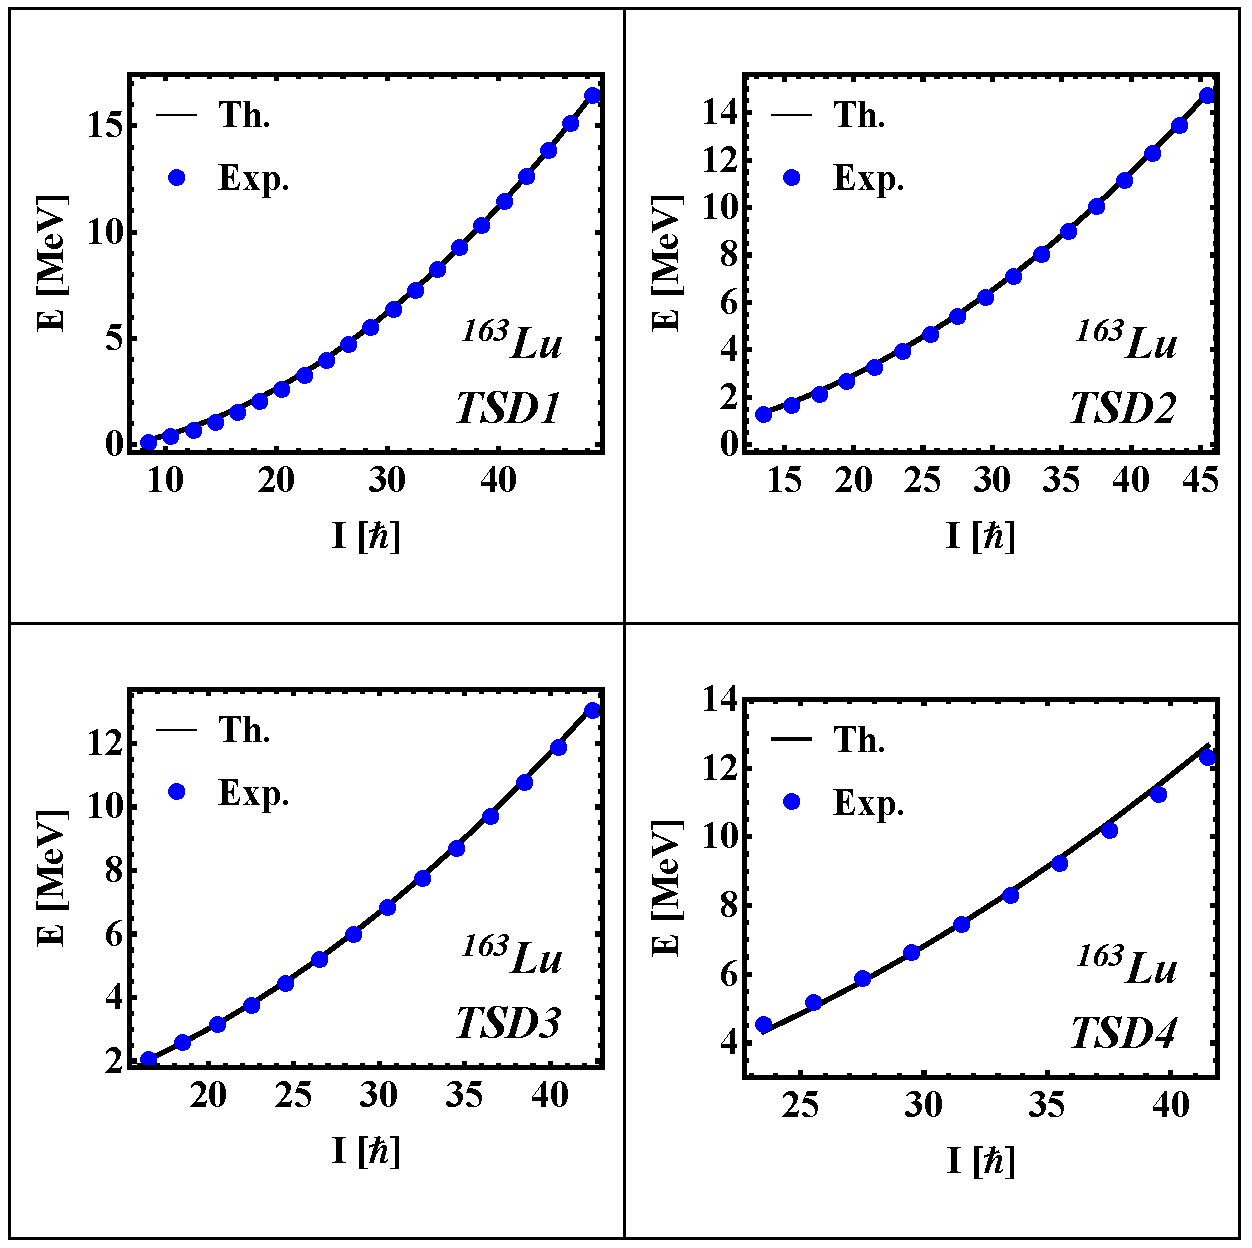
\includegraphics[scale=0.30]{ExcitationEnergies_GridView.eps}
    \caption{The excitation energies for the bands TSD1, TSD2, TSD3, and TSD4. }
    \label{tsd_bands}
\end{figure}

In terms of the stability of the wobbling motion with respect to the total angular momentum, several contour plots were plotted, using the obtained parameter set $\mathcal{P}$ with the help of Eq.  \ref{energy_function}.  For each band, a spin close to the band head of each sequence was chosen.  Due to the obtained MOI ordering, the surfaces have minimum points indicated by the red dots for each figure.  Results can be seen in Figs.  \ref{contour-tsd1},\ref{contour-tsd3}.  The four figures have many similarities suggesting common collective properties, but also differences caused by the fact that minima have different depths. The common feature consists of that the equi-energy curves surround a sole minimum for low energy while for higher energies the trajectories go around all minima, the lack of localization indicating an unstable picture. 

\begin{figure}
    \centering
    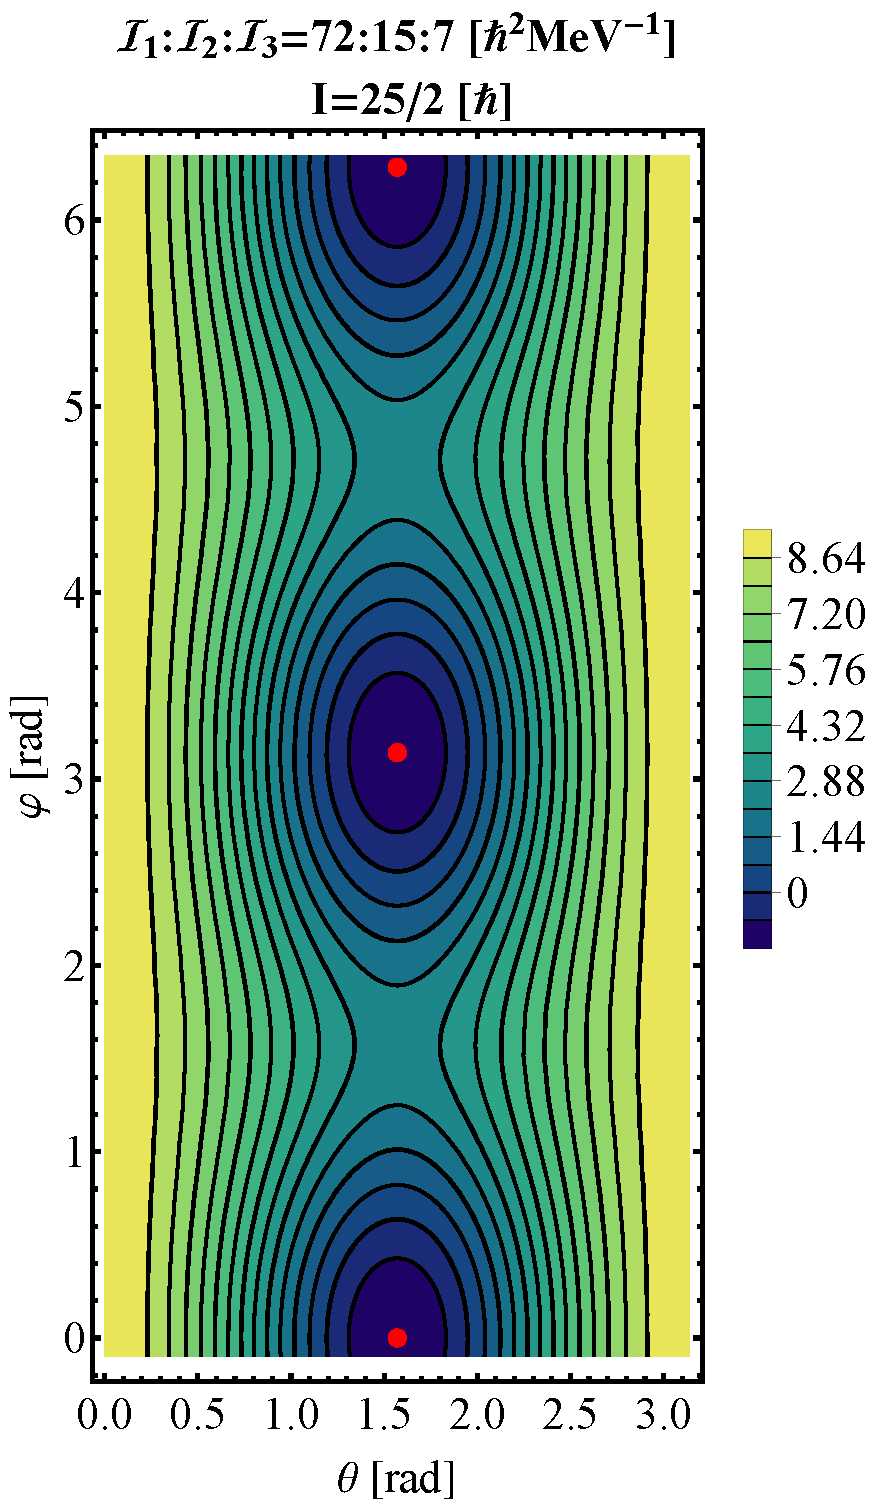
\includegraphics[scale=0.4]{contour-tsd1.eps}
    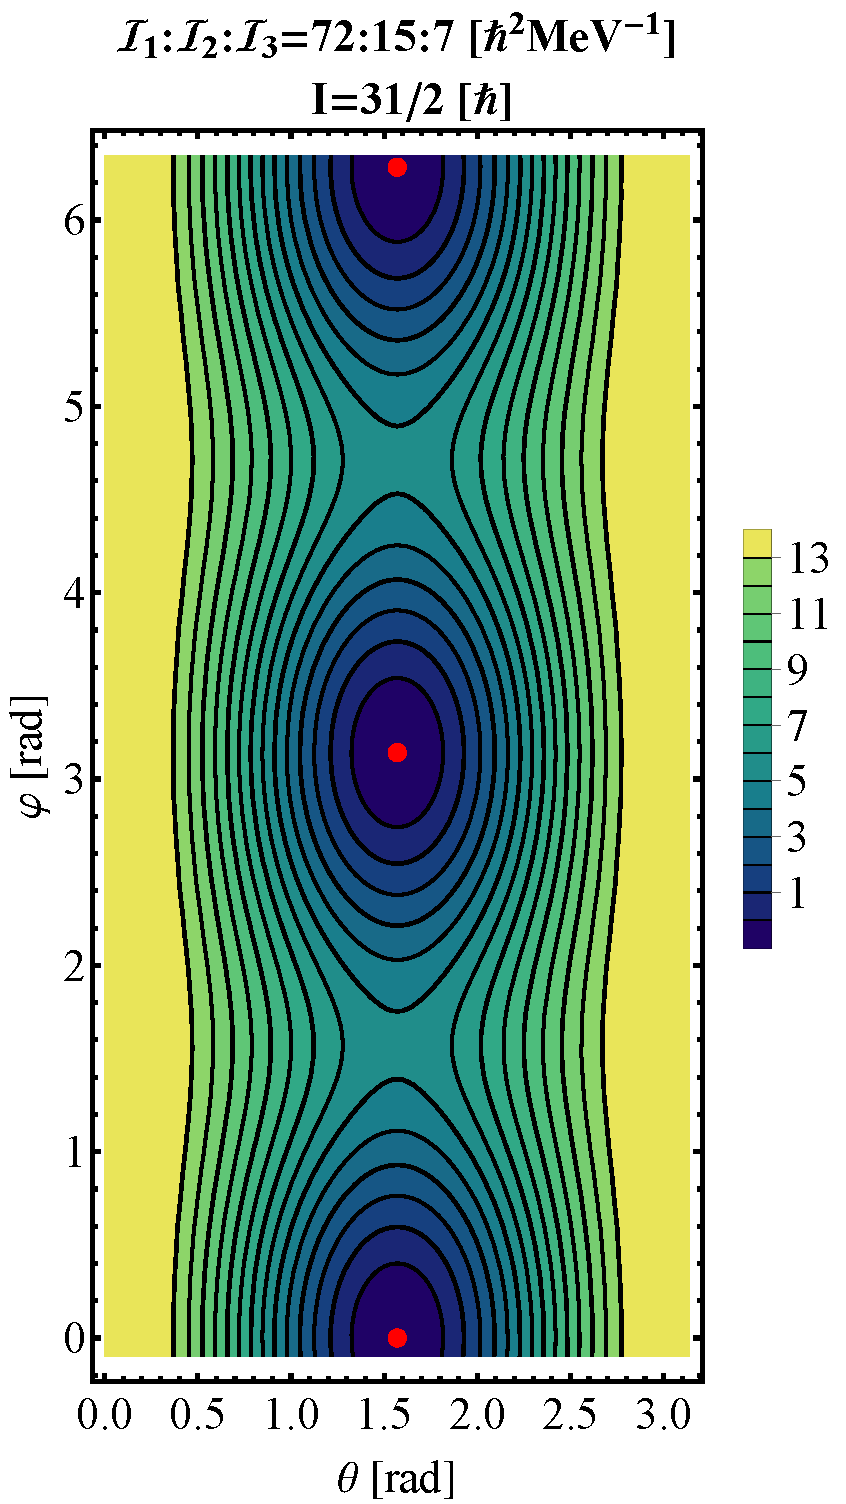
\includegraphics[scale=0.4]{contour-tsd2.eps}
    \caption{A contour plot with the energy function $\mathcal{H}$ for TSD1 and TSD2.  The parameter set $\mathcal{P}$ was used for the numerical calculations. }
    \label{contour-tsd1}
\end{figure}


\begin{figure}
    \centering
    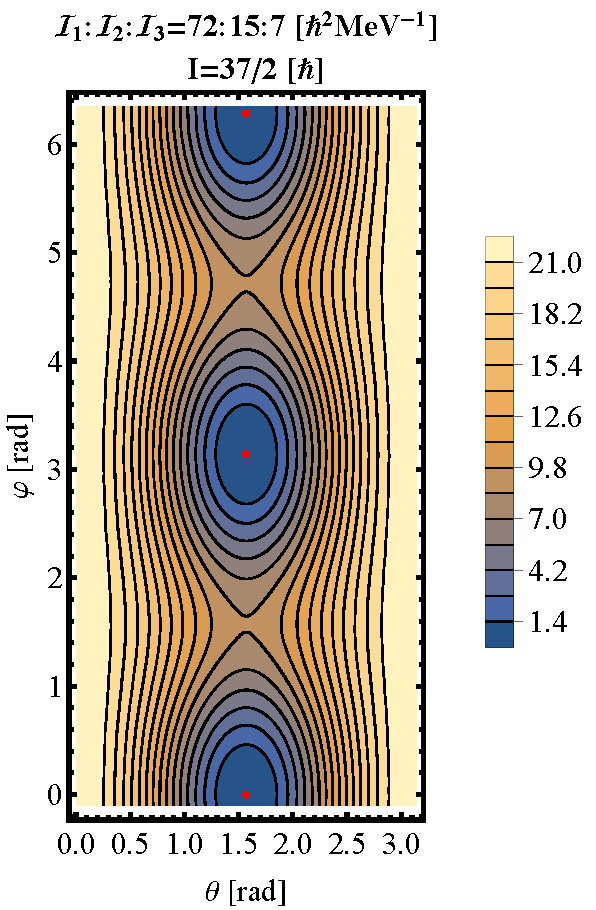
\includegraphics[scale=0.4]{contour-tsd3.eps}
    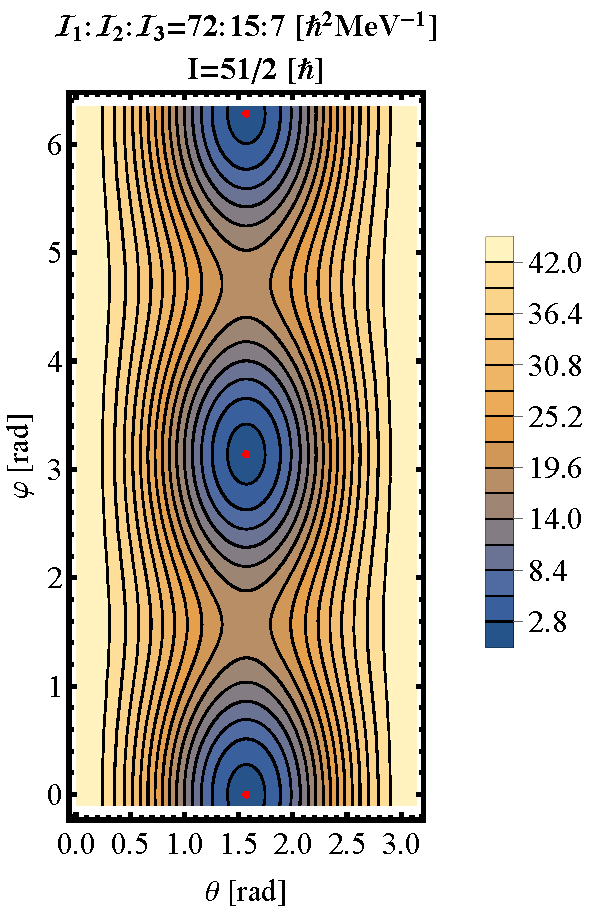
\includegraphics[scale=0.4]{contour-tsd4.eps}
    \caption{A contour plot with the energy function $\mathcal{H}$ for TSD3 and TSD4.  The parameter set $\mathcal{P}$ was used for the numerical calculations. }
    \label{contour-tsd3}
\end{figure}

Finally we are interested in finding out the dependence of the classical trajectories on angular momenta as well as on energies.  Indeed, when the model Hamiltonian is diagonalized for a given I,  a set of $2I+1$ energies are obtained.  Therefore, it makes sense to study the trajectory change at increasing the energy. Trajectories are represented as the manifold given by intersecting the surfaces corresponding to the two constants of motion.  The first energy in each row corresponds to the real excitation energy  for that particular spin state, the second one represents the point at which the ellipsoid touches the sphere at the equator, which marks a nuclear phase transition - while the third one is the trajectory of the system at energies sufficiently large that the system changes its wobbling regime.  For low energies, one notices two distinct trajectories having as rotation axes the 1-axis and -1-axis, respectively.  As energy increases the two trajectories approaches each other which results a tilted rotation axis for each of trajectories, the rotation axes being dis-aligned.  Note that this picture is fully consistent with that of Ref. \cite{Lawr}. When the two trajectories intersect each other, the trajectories surround both minima.  Increasing the energy even more one arrives again at two trajectories regime but with different rotation axes which become close to the 3-axis.  This reflects another phase transition for the system. 

\begin{figure}
    \centering
    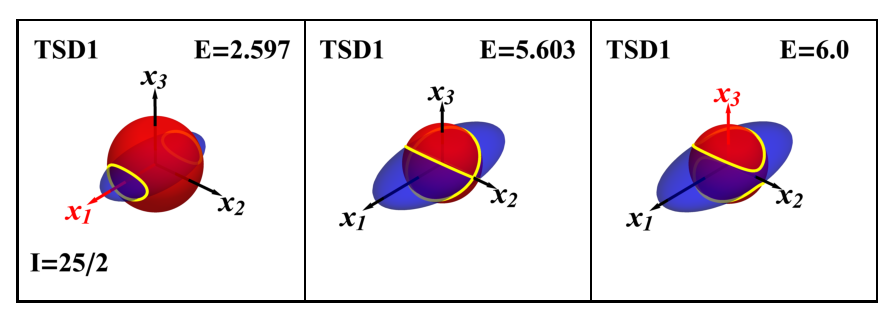
\includegraphics[scale=0.55]{tsd1_spin1.eps}
    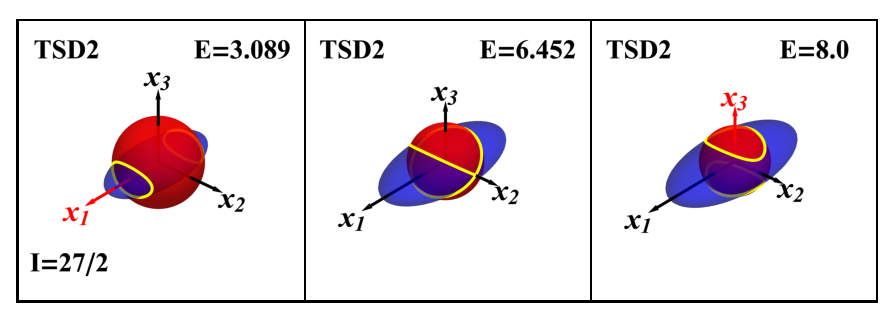
\includegraphics[scale=0.55]{tsd2_spin1.eps}
    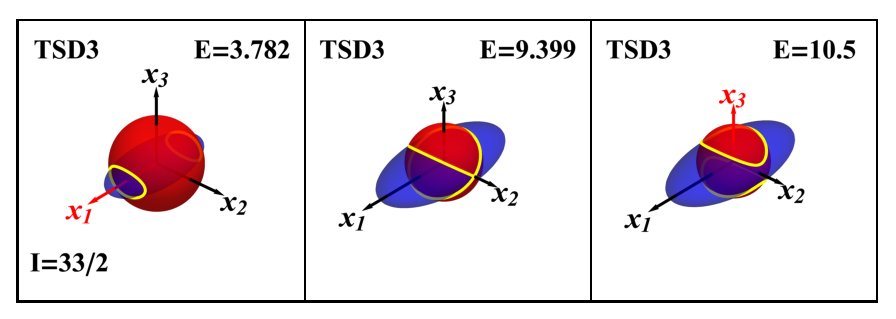
\includegraphics[scale=0.55]{tsd3_spin1.eps}
    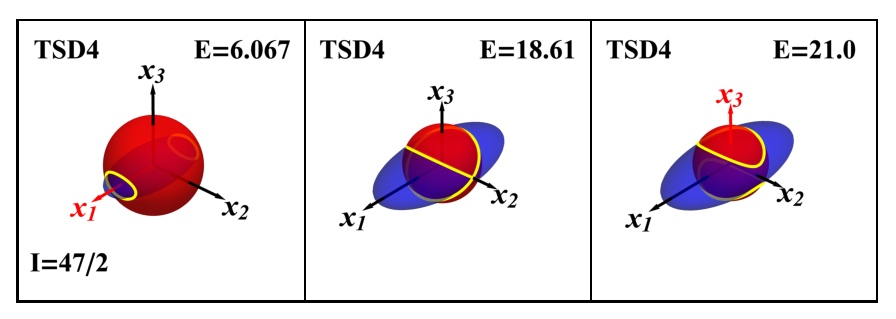
\includegraphics[scale=0.55]{tsd4_spin1.eps}
    \caption{The nuclear trajectory of the system for a spin state belonging to each of the four TSD bands of $^{163}$Lu.  Intersection line marked with yellow color represents the actual orbits. }
    \label{ellipsoids-tsd1}
\end{figure}

%\section{Conclusions}
The results of our investigation can be summarized as follows.  Despite the fact that TSD4 is of an opposite parity than the lower bands, the four bands are described by coupling a sole single particle of positive parity to the core states of positive parity for $TSD_{1,2,3}$ and negative parity for $TSD_4$.  The core is not changing, which results in having a unique set of MoI-s but the mean field for the valence nucleon is modified for unfavored signature as well as for the negative parity bands.  The contour plots for one representative state from each band, shows a similar structure but different depths and reaching the unstable regimes at different energies.  The system's trajectories corresponding to the four bands, obtained by intersecting the surfaces associated to the two constants of motion, the energy and the a. m. , indicate that for low energy the rotation axes are the 1-axis and -1-axis defining two disjoint trajectories, while for higher energy the rotation axes are tilted toward the 3-axis. There are signals that $TSD_2$ and $TSD_4$ are parity partner bands.  Likewise the bands $TSD_1$ and $TSD_2$ are signature partner bands.  The e. m.  properties of these bands have been successfully described in Ref. \cite{raduta2020new}.  Obviously, the results from the quoted paper are valid also here. 

Concluding, the present model is a successful tool for accurately describing the wobbling spectrum of $^{163}$Lu, but also for understanding the rotational motion of the nuclear system with respect to its total spin. 

{\bf Acknowledgments}. This work was supported by UEFISCU through the project PCE- PN3/2021

%\section{Acknowledgments}
\begin{thebibliography}{99}
\bibitem{BMott}A.  Bohr and B.  Mottelson, {\it Nuclear Structure} (Benjamin, Reading, MA, 1975), Vol.  II, Ch.  4. 
\bibitem{odegaard2001evidence},S.  W.  {\O}deg{\aa}rd, {\it et al. }, Phs.  Rev.  Lett. {\bf 86} 5866, (2001). 
\bibitem{Jens} D.  R.  Jensen {\it et al. }, Nucl.  Phys.  {\bf A 703}, 3, (2002). 
\bibitem{Scho} G.  Schoenwasser {\it et al. }, Phys.  Lett.  {\bf B 552},9, (2003). 
\bibitem{Amro} H.  Amro {\it et al. }, Phys.  Lett.  {\bf B 553}, 197, (2003). 
\bibitem{Hage}G.  B.  Hagemann, Eur.  Phys.  J.  {\bf A 20}, 183, (2004). 
\bibitem{Hage1} G.  B.  Hagemann {\it et al. }, Phys.  Rev.  Lett.  86, 5866 (2001). 
\bibitem{Matta} J.  T.  Matta {\it et al. }, Phys.  Rev.  Lett.  {\bf 114}, 082501 (2015). 
\bibitem{Sen}N.  Sensharma, {\it et al. },Phys.  Lett.  B,{\bf 792} (2019). 
\bibitem{Bring}P.  Bringel {\it et al. } Eur.  Phys.  J.  {\bf A 24}, 167, (2005). 
\bibitem{Hart} D.  J.  Hartley {\it et al. }, Phys.  Rev.  {\bf C 80}, 041304(R), (2009).  
\bibitem{Sen1}N.  Sensharma, {\it et al. }, Phys.  Rev.  Lett.  {\bf 124}, 052501 (2020). 
\bibitem{Chen} Q.  B.  Chen, S.  Frauendorf and C.  M.  Petrache, Phys.  Rev.  C {\bf 100}, 061301(R) (2019). 
\bibitem{Timar} J.  Timar {\it et al. }, Phys.  Rev.  Lett.  {\bf 122}, 062501 (2019). 
\bibitem{Chakr}S.  Chakraborty {\it et al. },Phys.  Lett.  B, {\bf 811} , 135854 (2020). 
\bibitem{Nand} S.  Nandi,{\it et al. },Phys.  Rev.  Lett.  {\bf 125} 132501 (2020). 
\bibitem{frauendorf2014transverse} S.  Frauendorf and F.  D\"{o}nau Phys.  Rev.  C {\bf 89}, 014322 (2014). 
\bibitem{raduta2020towards} A.  A. Raduta, R.   Poenaru, R and C.  M.  Raduta Jour.  Phys.  G:Nucl.  Part.  Phys. {\bf 47},025101 (2020).  
\bibitem{raduta2020new} A.  A.  Raduta, R.  Poenaru, R and C.  M.  Raduta, Phys.  Rev.  C {\bf 101}, 014302,(2020). 
\bibitem{Davyd} A. C.  Davydov, {\it Teoria atomnova yadra}, Moscva, 1958 (in russian), chapters 19,20. 
\bibitem{raduta2016specific} A.  A.  Raduta, Prog.  Part.  Nucl.  Phys.  {\bf 90, 241 (2016}. 
\bibitem{raduta2017semiclassical} A.  A. Raduta, R.  Poenaru, and L.  Gr.  Ixaru, Phys.  Rev.  C {\bf 96}, 054320, (2017). 
\bibitem{Buda} R.  Budaca, Phys.  Rev.  C {\bf 97} 069801 (2018). 
\bibitem{chas}R.  R.  Chasman, Phys. Lett.  B {\bf 96},7,(1980). 
\bibitem{Rad1}A.  A.  Raduta, Al.  H.  Raduta and Amand Faessler, Phys.  Ref.  C {\bf 55}, 1747, 91997). 
\bibitem{Rad2}A.  A.  Raduta, D.  Ionescu and Amnd Faessler, Phys.  Rev.  C {\bf 65}, 233 (2002). 
\bibitem{Rad3}A.  A.  Raduta, Al.  H.  Raduta and C.  M.  Raduta, Phys.  Rev.  C {\bf 74} 044312 (2006). 
\bibitem{Lawr} E.  A.  Lawrie, O, Shirinda and C.  M.  Petrache, Phys.  Rev.  C {\bf 101}, 034306 (2020). 
\end{thebibliography}  
\end{document}
%%%%%%%%%%%%%%%%%%%%%%%%%%%%%%%%%%%%%%%%%%%%%%%%%%%%%%%%%%%%%%%%%%%%%%%%%%%%%%%%%%%%%%%%%%%%%%%%%%%%%%%%%%%%%%%%%%%%



Jens,Scho,Amro,Hage,Bring,Hage1}
\cite{Jens,Scho,Amro,Hage,Bring,Hage1}, $^{167}$Ta \cite{Hart}, $^{135}$Pr  
\cite{Tan017,Tana018,Frau,Frau018,Buda,Matta,Sen}, $^{187}$Au \cite{Sen1}, $^{133}$La\cite{Biswas}, $^{105}$Pd \cite{Timar} and $^{133}$Ba \cite{Devi}. 
\begin{thebibliography}{99}
\bibitem{BMott}A.  Bohr and B.  Mottelson, {\it Nuclear Structure} (Benjamin, Reading, MA, 1975), Vol.  II, Ch.  4. 
\bibitem{Marsh}E.  R.  Marshalek, Nucl.  Phys.  {\bf A 331}, 429, (1979). 
\bibitem{Odeg}S.  W.  Odegard, {\it et al. }, Phys.  Rev.  Lett.  {\bf 86}, 5866, (2001). 
\bibitem{Jens} D.  R.  Jensen {\it et al. }, Nucl.  Phys.  {\bf A 703}, 3, (2002). 
\bibitem{Ikuko}I.  Hamamoto {\it et al. } Acta.  Phys.  Pol.  {\bf B32}, 2545, (2001).  
\bibitem{Scho} G.  Schoenwasser {\it et al. }, Phys.  Lett.  {\bf B 552},9, (2003). 
\bibitem{Amro} H.  Amro {\it et al. }, Phys.  Lett.  {\bf B 553}, 197, (2003). 
\bibitem{Gorg} A.  G\"{o}rgen et al. , Phys.  Rev {\bf C 69}, 031301(R), (2004). 
\bibitem{Ham} I.  Hamamoto, Phys.  Rev.  {\bf C 65}, 044305, (2002). 
\bibitem{Matsu} M.  Matsuzaki, Y.  R.  Shimizu, K.  Matsuyanagi, Phys.  Rev.  {\bf C 65}, 041303(R), (2002);
Yoshifumi R.  Shimizu, Masayuki Matsuzaki and Kenichi Matsuyanagi,arXiv:nucl-th/0404063v1, 22 Apr.  2004. 
\bibitem{Ham1}I.  Hamamoto and G.  B.  Hagemann, Phys.  Rev.  {\bf C 67}, 014319, (2003). 
\bibitem{Jens1} D.  R.  Jensen {\it et al. }, Eur.  Phys.  J.  {\bf A 19}, 173, (2004). 
\bibitem{Hage}G.  B.  Hagemann, Eur.  Phys.  J.  {\bf A 20}, 183, (2004). 
\bibitem{Tana3}K.  Tanabe and K.  Sugawara-Tanabe, Phys.  Rev.  {\bf C73},  034305, (2006).  
\bibitem{Oi} Makito Oi, Phys.  Lett.  {\bf B 634}, 30 (2006). 
\bibitem{Rad07}A.  A.  Raduta, R.  Budaca and C.  M.  Raduta,  Phys.  Rev.  C,  {\bf 76}, 064309,(2007). 
\bibitem{Bring}P.  Bringel {\it et al. } Eur.  Phys.  J.  {\bf A 24}, 167, (2005). 
\bibitem{Hage1} G.  B.  Hagemann {\it et al. }, Phys.  Rev.  Lett.  86, 5866 (2001). 
\bibitem{Hart} D.  J.  Hartley {\it et al. }, Phys.  Rev.  {\bf C 80}, 041304(R), (2009).  
\bibitem{Cast}R. F.  Casten, E.  A.  McCutchan, N.  V.  Zamfir, C.  W.  Beausuang and Jing-ye Zhang,
Phys.  Rev.  {\bf C 67}, 064306, (2003). 
\bibitem{Alme} D.  Almehed, R.  G.  Nazmitdinov and F.  D\"{o}nau, Phys.  Scr.  {\bf T125}, 139, (2006). 
\bibitem{MikIans} I.  N.  Mikhailov and D.  Janssen, Phys.  Lett.  {\bf 72B}, 303, (1978). 
\bibitem{Rad016}A.  A.  Raduta, Progress in Particle and Nuclear Physics 90, 241, (2016). 
\bibitem{Badea} M. Badea and A.  A.  Raduta, Rev.  Roum.  Phys.  21 , 743, (1979). 
\bibitem{Rad017}A.  A.  Raduta, R.  Poenaru and L.  Gr.  Ixaru, Phys.  Rev.  C {\bf 96}, 054320, (2017). 
\bibitem{Rad018}A.  A.  Raduta, R.  Poenaru and Al.  H.  Raduta, J.  Phys.  G: Nucl.  Part.  Phys.  {\bf 45} 105104 (2018). 
\bibitem{Rad20} A.  A.  Raduta, R Poenaru and C M Raduta, J.  Phys.  G: Nucl.  Part.  Phys.  {\bf 47},025101 (2020). 
\bibitem{Rad201} A.  A.  Raduta, R Poenaru and C M Raduta, Phys.  Rev.  C {\bf 101}, 014302 (2020). 
\bibitem{Tan017} Kosai Tanabe and Kazuko Sugawara Tanabe, Phys.  Rev.  C {\bf 95},  064315, (2017). 
\bibitem{Tana018} Kosai Tanabe and Kazuko Sugawara Tanabe, Phys.  Rev.  C {\bf 97},069802 (2018). 
\bibitem{Frau} S.  Frauendorf and F.  Donau, Phys.  Rev.  C {\bf 89},014322, (2014). 
\bibitem{Frau018} S.  Frauendorf, Phys.  Rev.  {\bf C97}, 069801 (2018). 
\bibitem{Buda} R.  Budaca, Phys.  Rev.  C {\bf 97}, 024302, (2018). 
\bibitem{Matta} J.  T.  Matta {\it et al. }, Phys.  Rev.  Lett.  {\bf 114}, 082501 (2015). 
\bibitem{Sen} N.  Sensharma {\it et al. },Phys.  Lett.  B {\bf 792}, 170 (2019). 
\bibitem{Sen1} N.  Sensharma {\it et al. },Phys.  Rev.  Lett.    {\bf 124}, 052501 (2020). 
\bibitem{Biswas} S.  Biswas {\it et al. },European Physical Journal A, 5, 12856 (2019).  
\bibitem{Timar} J.  Timar {\it et al. }, Phys.  Rev.  Lett.  {\bf 122}, 062501 (2019). 
\bibitem{Devi} K.  Rojeeta Devi, Proc.  of the DAE Symp.  on Nucl.  Phys.  62, 308 (2017). 
\bibitem{Chen1} Q. P. Chen,S.  Q.  Zhang and J.  Meng, Phys.  Rev.  {\bf C 94}, 054308 (2016). 
\bibitem{Lawr} E.  A.  Lawrie, O, Shirinda and C.  M.  Petrache, Phys.  Rev.  C {\bf 101}, 034306 (2020). 
\bibitem{HolPr} T.  Holstein and H.  Primakoff, Phys.  Rev.  {\bf 58}, 1098 (1940). 
\bibitem{Dys} T.  F.  Dyson, Phys.  Rev.  {\bf 102},1217 (1958). 
\bibitem{Bar}V.  Bargmann, Rev.  Mod.  Phys.  {\bf 34}, 829(1962). 
\bibitem{Gold}J.  Goldstone, Nuovo Cimento {\bf 19}, 154 (1961). 
\bibitem{Davy} A. S.  Davydov and G. F.  Filippov, Nucl.  Phys.  {\bf 8}, 788, (1958). 
\bibitem{WilJean} L.  Wilets and M.  Jean, Phys.  Rev.  {\bf 102}, 788 (1956). 
\bibitem{TerVehn} J.  Meyer-ter-Vehn, Nucl.  Phys.  {\bf A249}, 111, 141, (1975). 
\bibitem{Bona2} D.  Bonatsos, D.  Lenis, D.  Petrellis and P.  A.  Terziev, Phys.  Lett.  {\bf B 588} 172,(2004). 
\bibitem{Bona3} D.  Bonatsos, D.  Lenis, D.  Petrellis, P.  A.  Terziev and I.  Yigitoglu, Phys.  Lett.  {\bf B 621},  102, (2005). 
\bibitem{Rad09}A.  A.  Raduta, {\it et al. }, Nucl.  Phys.  {\bf A 819}, 46 (2009). 
\bibitem{Davyd} A. C.  Davydov, {\it Teoria atomnova yadra}, Moscva, 1958 (in russian), chapters 19,20. 
\bibitem{Toki1}H.  Toki and Amand Faessler, Nucl.  Phys.  {\bf A 253}, 231 (1975). 
\bibitem{Toki2}H.  Toki and Amand Faessler, Z.  Physik {\bf A 276}, 35 (1976). 
\bibitem{Toki3}H.  Toki and Amand Faessler, Phys.  Lett.  {\bf B 63}, 121 (1976). 
\bibitem{Toki4}H.  Toki, K.  Neergard, P.  Vogel, and Amand Faessler, Nucl.  Phys.  {\bf A 279}, 1 (1977). 
\bibitem{Toki5}H.  Toki, H.  L.  Yadav, A.  Faessler, Phys.  Lett.  {\bf B 66}, 310 (1977). 
\bibitem{Ogu}T.  Oguchi, Progr.  Th.  Phys, {\bf 25},721 (1961). 
\bibitem{Rad98}A.  Gheorghe, A.  A.  Raduta, V.  Ceausescu,  Nucl.  Phys.  A 637, 201, (1998). 
\bibitem{Rose}M.  E.  Rose, {\it Elementary Theory of Angular Momentum} (Wiley, New York, 1957). 
\bibitem{Jol}D.  Janssen, F.  Donau, S.  Frauendorf and R.  V.  Jolos, Nucl.  Phys.  {\bf A 172}, 145 (1971). 
\bibitem{Rad74}V.  Ceausescu, A.  A.  Raduta, Prog.  Th.  Phys.  {\bf 52} (3), 903 (1974)
\bibitem{Rad91} A. A. Raduta, A. Faessler and S. Stoica.  Nucl. Phys. A 534, 149, (1991).  
\bibitem{Klein91} A.  Klein and E.  R.  Marshalek, Rev.  Mod.  Phys.  {\bf 63}, 375 (1991). 
\end{thebibliography}
\end{document}







